%%%% Proceedings format for most of ACM conferences (with the exceptions listed below) and all ICPS volumes.
\documentclass[sigconf]{acmart}
%%%% As of March 2017, [siggraph] is no longer used. Please use sigconf (above) for SIGGRAPH conferences.

%%%% Proceedings format for SIGPLAN conferences 
% \documentclass[sigplan, anonymous, review]{acmart}

%%%% Proceedings format for SIGCHI conferences
% \documentclass[sigchi, review]{acmart}

%%%% To use the SIGCHI extended abstract template, please visit
% https://www.overleaf.com/read/zzzfqvkmrfzn

%
% defining the \BibTeX command - from Oren Patashnik's original BibTeX documentation.
\def\BibTeX{{\rm B\kern-.05em{\sc i\kern-.025em b}\kern-.08emT\kern-.1667em\lower.7ex\hbox{E}\kern-.125emX}}
    
% Rights management information. 
% This information is sent to you when you complete the rights form.
% These commands have SAMPLE values in them; it is your responsibility as an author to replace
% the commands and values with those provided to you when you complete the rights form.
%
% These commands are for a PROCEEDINGS abstract or paper.
\copyrightyear{2019}
\acmYear{2019}
\setcopyright{acmlicensed}
\acmConference[Web3D '19]{24th International ACM Conference on 3D Web Graphics and Interactive Technology (Web3D 2019),}{July 26--28, 2019}{Los Angeles, CA}
\acmBooktitle{24th International ACM Conference on 3D Web Graphics and Interactive Technology (Web3D 2019), July 26--28, 2019, Los Angeles, CA}
\acmPrice{150.00}
\acmDOI{10.1145/0000.0000}
\acmISBN{000-000-000}

%
% These commands are for a JOURNAL article.
%\setcopyright{acmcopyright}
%\acmJournal{TOG}
%\acmYear{2018}\acmVolume{37}\acmNumber{4}\acmArticle{111}\acmMonth{8}
%\acmDOI{10.1145/1122445.1122456}

%
% Submission ID. 
% Use this when submitting an article to a sponsored event. You'll receive a unique submission ID from the organizers
% of the event, and this ID should be used as the parameter to this command.
%\acmSubmissionID{123-A56-BU3}

%
% The majority of ACM publications use numbered citations and references. If you are preparing content for an event
% sponsored by ACM SIGGRAPH, you must use the "author year" style of citations and references. Uncommenting
% the next command will enable that style.
%\citestyle{acmauthoryear}

\usepackage{subcaption}
% \usepackage{minted}
\usepackage{caption}
\usepackage[newfloat]{minted}
\captionsetup[listing]{position=top}

% add some settings to dramatically reduce hypenation
\pretolerance=5000
\tolerance=9000
\emergencystretch=0pt
\righthyphenmin=4
\lefthyphenmin=4
%
% end of the preamble, start of the body of the document source.
\begin{document}

%
% The "title" command has an optional parameter, allowing the author to define a "short title" to be used in page headers.
\title{A Practical Approach to Integrating Live 2D Web Content with the Immersive Web}

%
% The "author" command and its associated commands are used to define the authors and their affiliations.
% Of note is the shared affiliation of the first two authors, and the "authornote" and "authornotemark" commands
% used to denote shared contribution to the research.

\author{Gheric Speiginer}
% \authornote{}
\orcid{0000-0002-4770-8781}
\affiliation{%
  \institution{Georgia Institute of Technology}
  \streetaddress{North Avenue}
  \city{Atlanta}
  \state{Georgia}
  \postcode{30332}
}
\email{gheric@gatech.edu}

\author{Blair MacIntyre}
% \authornote{}
\affiliation{%
  \institution{Georgia Institute of Technology}
  \streetaddress{North Avenue}
  \city{Atlanta}
  \state{Georgia}
  \postcode{30332}
}
\affiliation{%
  \institution{Mozilla}
  \streetaddress{}
  \city{Mountain View}
  \state{California}
  \postcode{}
}
\email{blair@{gatech.edu, mozilla.com}}


%
% By default, the full list of authors will be used in the page headers. Often, this list is too long, and will overlap
% other information printed in the page headers. This command allows the author to define a more concise list
% of authors' names for this purpose.
\renewcommand{\shortauthors}{Speiginer and MacIntyre}

\lccode`3=`3
\hyphenation{WebLayer3D} % ERROR: 3 is not a letter. (it is now)
\hyphenation{WebGL WebXR}
\hyphenation{ARKit ARCore}


%
% The abstract is a short summary of the work to be presented in the article.
\begin{abstract}
 As 3D on the web gains momentum via standards such as WebGL and WebXR, a reoccurring frustration among web developers is the desire to leverage 2D web technologies within immersive presentation contexts. The use-cases for blending 2D and 3D web content include progressive enhancement of 2D web pages, re-use of existing 2D web content, and layout/design of complex interactive user interfaces for 3D environments. We introduce WebLayer3D, a JavaScript plugin for three.js (a popular 3D scene-graph library) that makes it easy for web developers to integrate live interactive 2D web content (built using standard web technologies) into a 3D scene (rendered using WebGL). In this paper, we demonstrate that existing DOM-to-Texture techniques (when used thoughtfully) are sufficient for enabling a performant, simple, and powerful approach to building complex interactive UIs for the immersive web.
\end{abstract}

%
% The code below is generated by the tool at http://dl.acm.org/ccs.cfm.
% Please copy and paste the code instead of the example below.
%
\begin{CCSXML}
<ccs2012>
<concept>
<concept_id>10003120.10003121.10003124.10010392</concept_id>
<concept_desc>Human-centered computing~Mixed / augmented reality</concept_desc>
<concept_significance>500</concept_significance>
</concept>
<concept>
<concept_id>10003120.10003121.10003124.10010866</concept_id>
<concept_desc>Human-centered computing~Virtual reality</concept_desc>
<concept_significance>500</concept_significance>
</concept>
<concept>
<concept_id>10003120.10003121.10003124.10010868</concept_id>
<concept_desc>Human-centered computing~Web-based interaction</concept_desc>
<concept_significance>500</concept_significance>
</concept>
<concept>
<concept_id>10003120.10003121.10003129.10011757</concept_id>
<concept_desc>Human-centered computing~User interface toolkits</concept_desc>
<concept_significance>500</concept_significance>
</concept>
</ccs2012>
\end{CCSXML}

\ccsdesc[500]{Human-centered computing~Web-based interaction}
\ccsdesc[500]{Human-centered computing~User interface toolkits}
\ccsdesc[500]{Human-centered computing~Virtual reality}
\ccsdesc[500]{Human-centered computing~Mixed/augmented reality}

%
% Keywords. The author(s) should pick words that accurately describe the work being
% presented. Separate the keywords with commas.
\keywords{web standards, rasterization, 3D user interfaces, webxr, webgl}

%
% A "teaser" image appears between the author and affiliation information and the body 
% of the document, and typically spans the page. 
\begin{teaserfigure}
  \begin{center}
  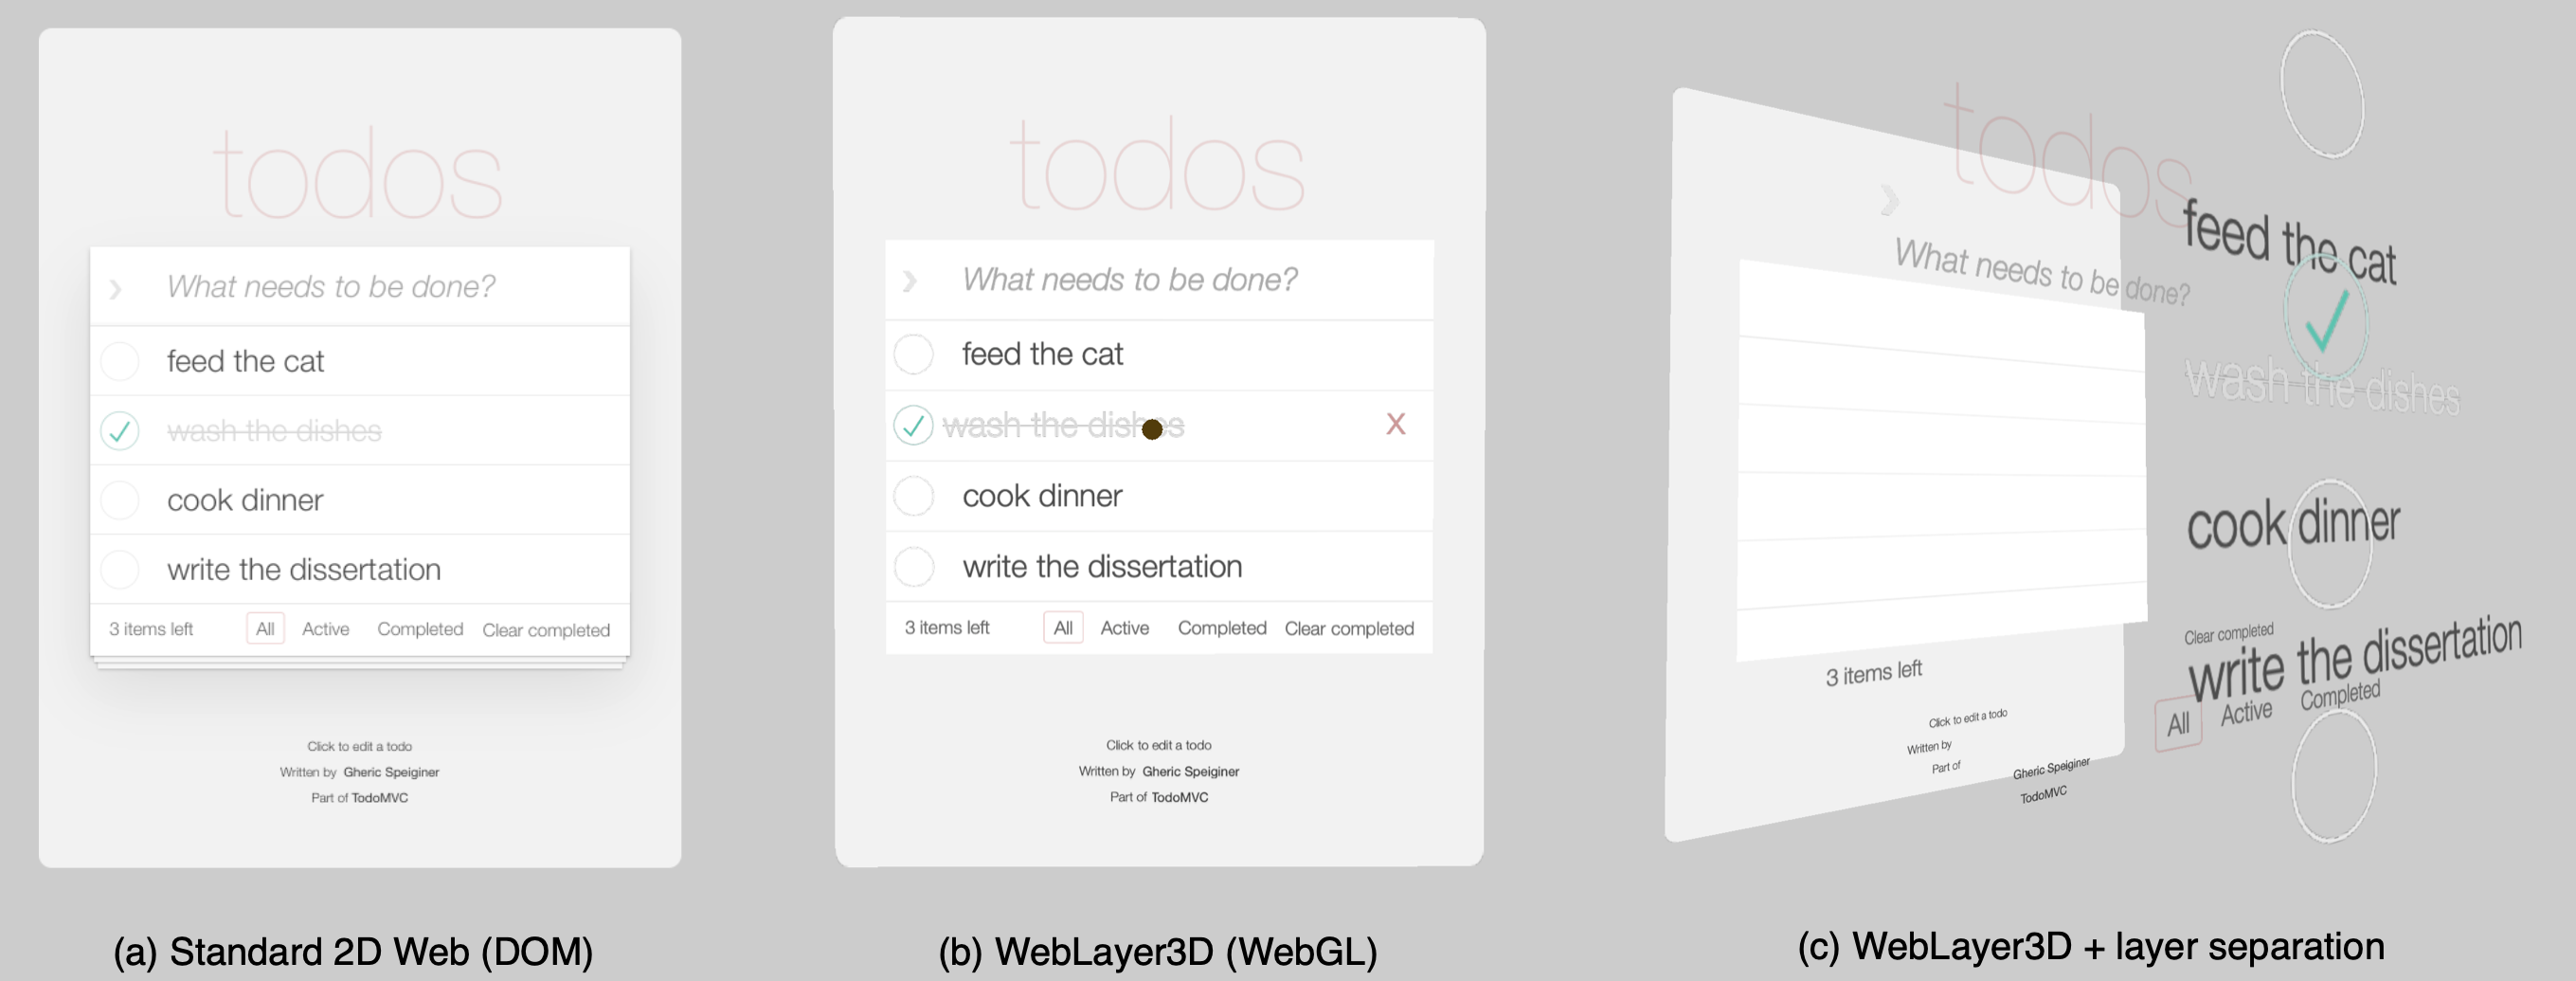
\includegraphics[width=\textwidth]{TodoMVC-Banner2.png}
  \end{center}
  \caption{The archetypal TodoMVC web application: (a) shows a typical web architecture (written in HTML/CSS/JavaScript, with the DOM managed by Vue.js) rendered natively by the browser; (b) is the same application, extended for rendering in WebGL using WebLayer3D, with a 3D cursor displayed for interaction (web content is rasterized using html2canvas and rendered as textured planes using three.js); (c) is the same scene viewed from an angle with the layers (the three.js objects) separated in 3D to create a kind of exploded view (for demonstration purposes). The UI remains fully interactive and responsive in both the 3D scene presentation and the underlying DOM presentation (they can be displayed and interacted with simultaneously).}
  \Description{}
  \label{fig:teaser}
\end{teaserfigure}

%
% This command processes the author and affiliation and title information and builds
% the first part of the formatted document.
\maketitle

\section{Introduction}
Not long ago, 3D graphics on the web (e.g., WebGL graphics displayed in \verb|<canvas>| elements) was something of a novelty, with limited vendor support and sparse use-cases. Today, however, WebGL is not only universally supported, but is quickly becoming a crucial component of the wider web ecosystem. With the advent of immersive systems (e.g., HTC Vive, Oculus Rift, Microsoft Hololens, etc.), computer-vision technologies (e.g., ARCore, ARKit, etc.), and up-coming web standards (e.g., WebXR), WebGL becomes a basic requirement for the immersive web. Unfortunately, these 3D web technologies are not fully inter-operable with traditional 2D web technologies (like HTML and CSS), leaving web developers building immersive applications unable to leverage much of their expertise, tools, or existing 2D web content. Even outside of a strictly web ecosystem (e.g., Unity and other popular game engines), the desire to build complex user-interfaces for immersive applications has frustrated developers who wish to leverage the web specifically for its powerful layout and styling capabilities. 

There are two primary use-cases for mixing together the 2D web and the immersive web: enabling users to surf and interact with legacy 2D web pages within an immersive presentation context (e.g., placing 2D web pages in floating windows in the 3D world), or leveraging 2D web elements and toolkits to create individual pieces of 2D web content for use within an immersive web application (e.g., building interactive 3D user-interfaces out of 2D web components). Our assumption is that operating systems and user-level shells on current and future XR devices will solve the former use case, providing access to full legacy 2D web content in their user-level interfaces (e.g., as Windows MR, Hololens and the Magic Leap ML1 currently do with their Edge and Helio web browsers). Therefore, our focus is on the latter use-case; specifically, our goal is to enable immersive applications to use the Document Object Model (DOM) and CSS Object Model (CSSOM) to create live, interactive 2D content elements that can be presented and manipulated in the 3D world. In particular, our approach is designed to allow developers to easily manipulate web content (however complex) in 3D, moving and arranging it as they see fit, while still leveraging the layout/styling capabilities of the DOM/CSSOM.

The key insight behind this work was that well designed 3D user-interfaces (UIs) will include 2D elements, but will rarely include a complex 2D UI presented in a rectangle and interacted with in the same way as a 2D UI on a flat screen (e.g., with scrolling boxes, drop down 2D menus, etc).  Instead, when developers and designers say they want to use HTML/CSS to create UI elements in 3D, they are really talking about using web layout and styling, along with some simple interactivity (such as hover-effects when the pointer moves over content, and click-event routing) to create \textit{2D content elements that can integrate into their 3D presentations}.  

For example, a large amount of text may be presented in a variety of ways in 3D, but a scrolling text box with a scroll bar in a fixed sized rectangle is not necessarily the best option; if the DOM can be used to lay out and style paragraphs of text, 3D developers can approach the task of presenting it to the user in many ways. Similarly, labels \cite{Tatzgern2014HedgehogSpace} and menu items \cite{BowmanDesignEnvironments} can be positioned, animated, and interacted with in many ways in 3D; the "pain point" for developers is creating beautiful 2D elements to use with these toolkits.  In these and other cases, integrating a collection of 2D DOM elements into the 3D environment, and supporting sending pointer and button events back to the 2D DOM, is one of the essential elements needed to ease the creation of beautiful 3D UIs. 

Our contribution, WebLayer3D\footnote{Available at https://github.com/argonjs/three-web-layer. The TodoMVC sample is included in this repository, and available to try out at https://argonjs.github.io/three-web-layer/}, simplifies that task of using the DOM to create the 2D content elements needed for 3D UIs, by allowing developers to
\begin{itemize}
\item organize (possibly complex) 2D elements within the DOM that are styled with standard CSS rules,
\item annotate the DOM to indicate which parts of the hierarchy might be moved independently in 3D,
\item automate the creation of a collection of \textit{three.js}\footnote{https://threejs.org} scene-graph objects from this annotated DOM,
\item pre-render multiple variations of the DOM to support hover effects and alternative styling specified via CSS classes and automatically use the appropriate version, 
\item interact with the DOM using whatever 3D pointing and manipulation techniques their application already uses, and
\item transition the view when the DOM structure changes, while supporting 2D DOM layout or custom spatial layout.
\end{itemize}

By not focusing on the harder problem of injecting entire (arbitrary) web pages into 3D, the issues and limitations that prevent arbitrary content from being rendered using DOM-to-Texture are avoided.  We assume developers are primarily interested in leveraging the layout and composition capabilities of HTML/CSS, and will create, arrange and annotate web content specifically for the purpose of presenting in their 3D UIs. WebLayer3D simplifies the process of importing live 2D web content into a 3D scene as a set of rasterized layers, and demonstrates how the 3D web can benefit from the power of the 2D Web for building complex (and performant) interactive user interfaces via DOM-to-Texture capabilities. Our approach enables immersive application developers to directly leverage HTML/CSS for layout and design, allowing for re-use and non-trivial integration of existing web content into a 3D environment. By relying on DOM rasterization, our approach remains simple and adaptable to future native DOM rasterization capabilities. 

In this paper, we discuss the problem of integrating 2D web content into a 3D scene, and how our approach relates to other approaches to this problem. We detail our implementation, including its limitations, and show examples of how it can be used as part of a real system to create adaptive 3D interfaces. We conclude with some ideas for future work in this area.

\section{Background and Related Work}


\begin{figure}[h]
  \centering
    \begin{subfigure}{0.65\linewidth}
    \centering
    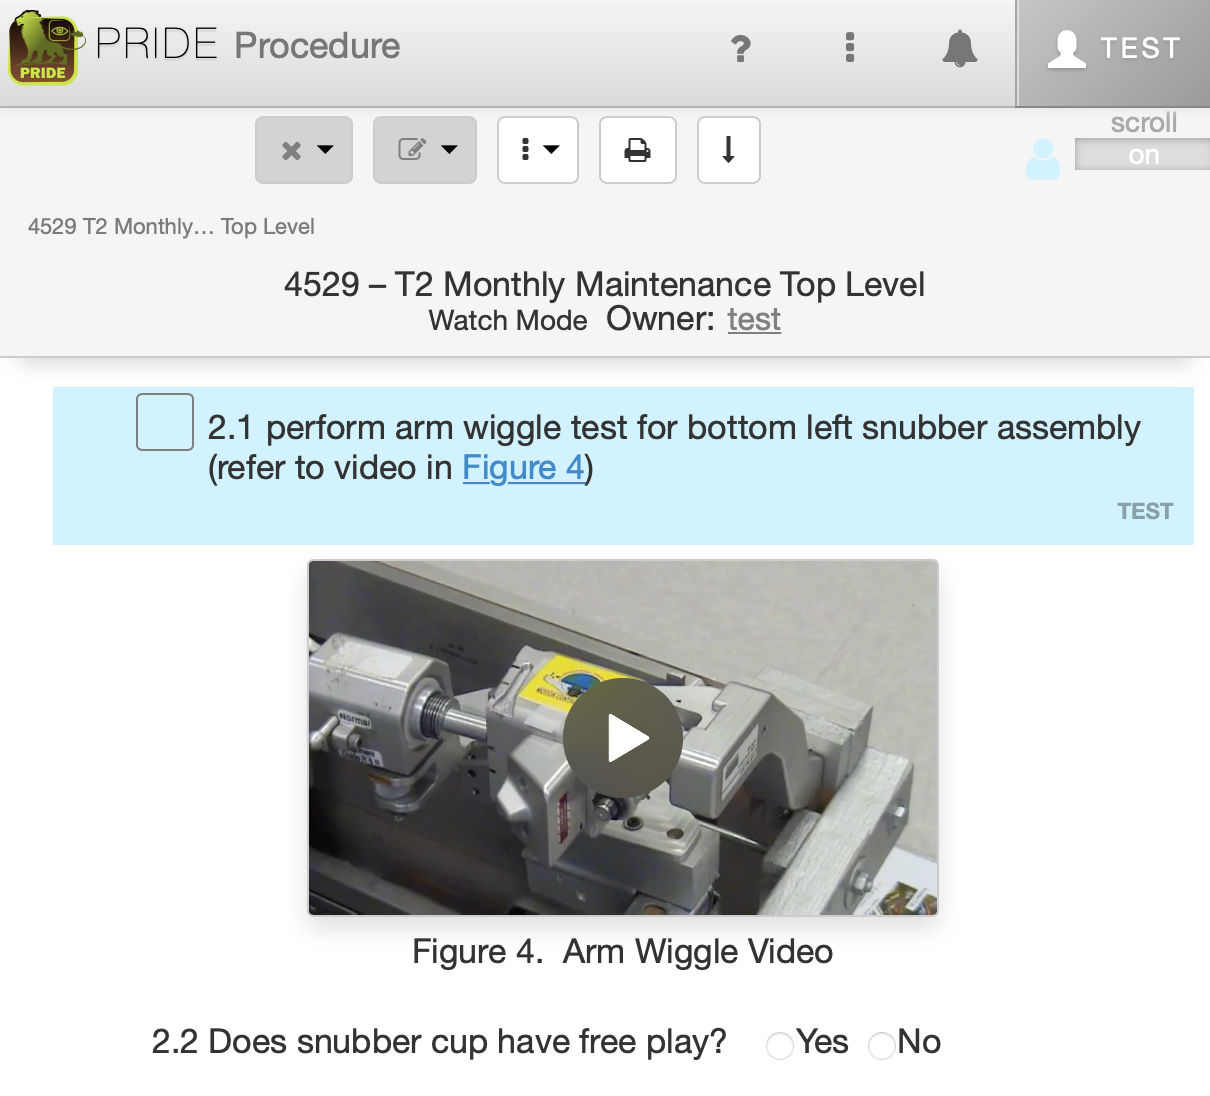
\includegraphics[width=\linewidth]{PRIDE-View.png}
    \end{subfigure}
    \begin{subfigure}{0.33\linewidth}
    \centering
    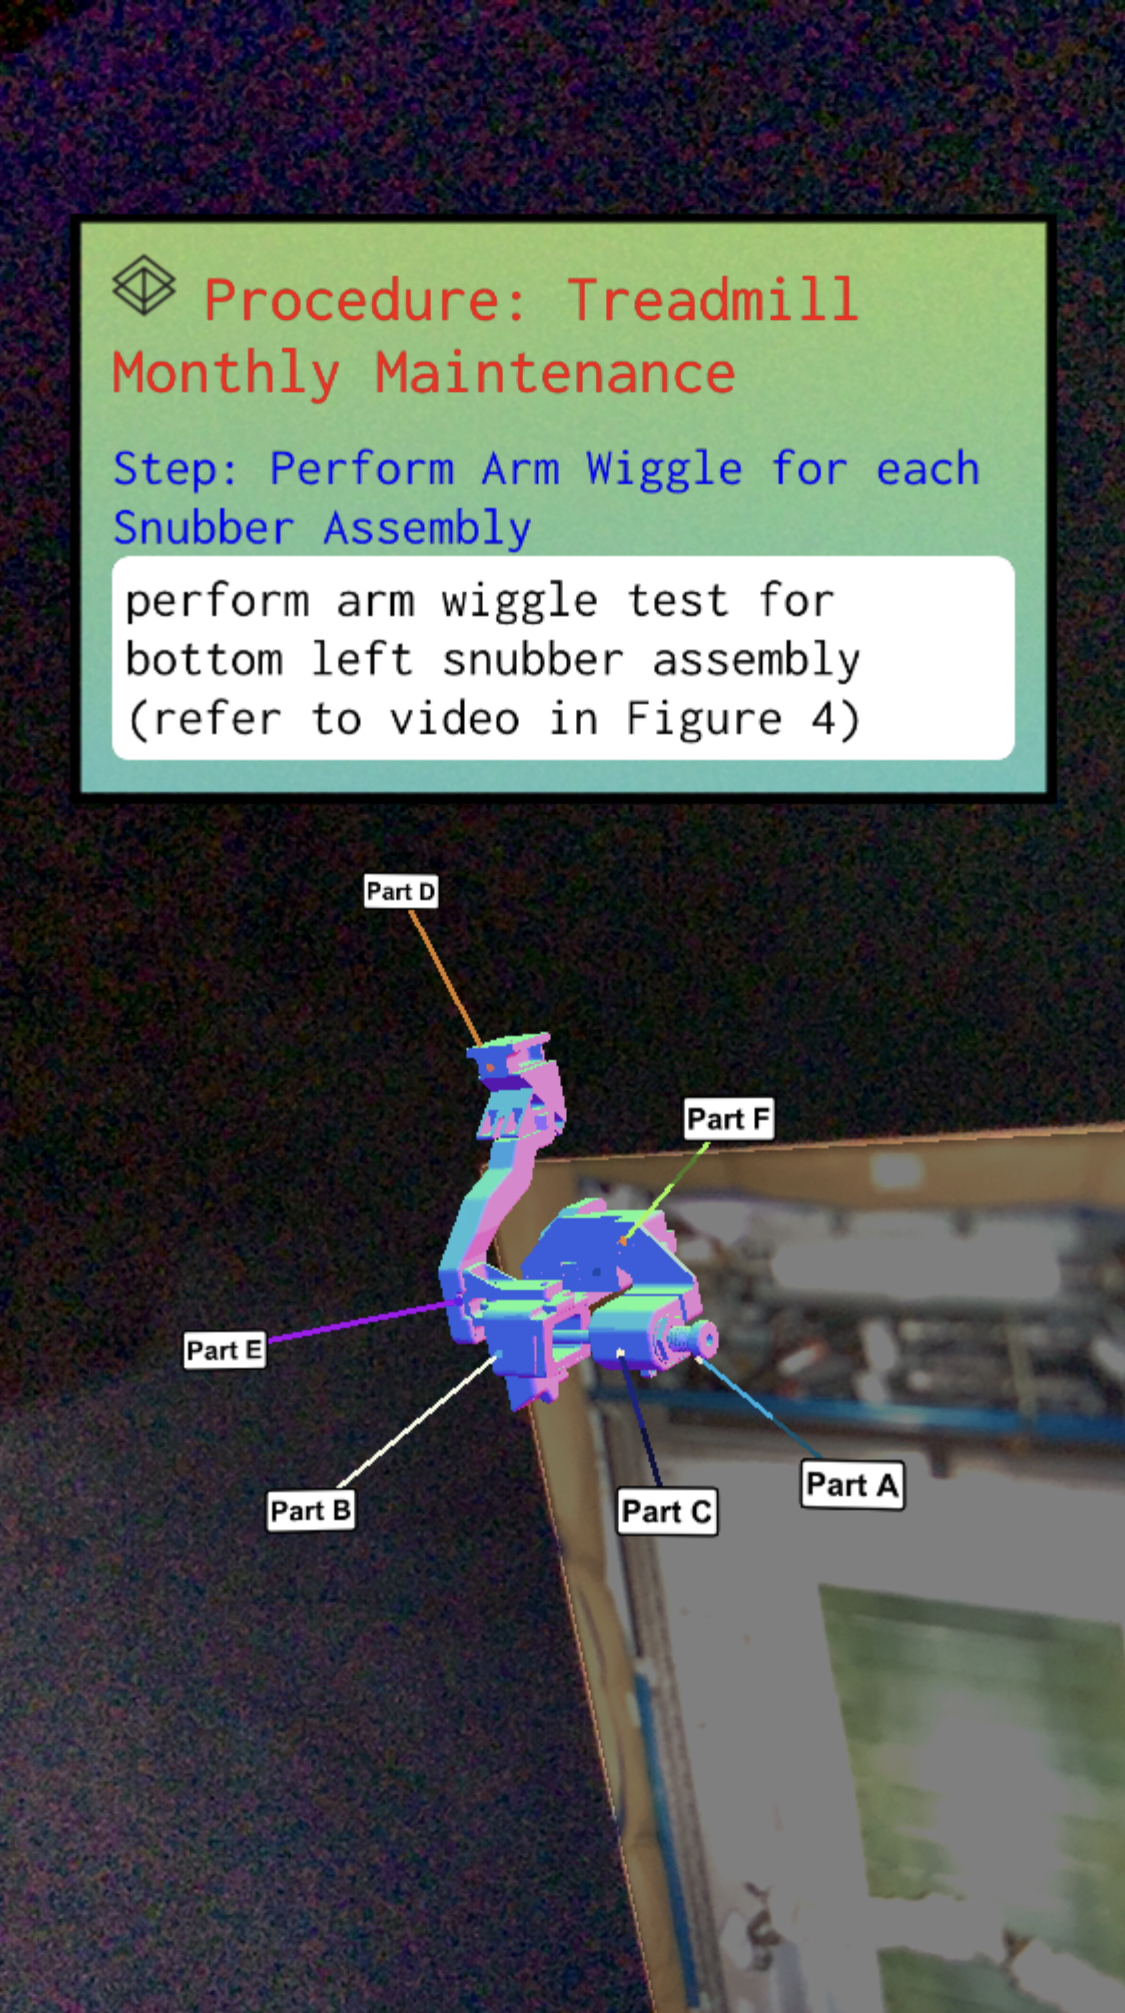
\includegraphics[width=\linewidth]{PRIDE-AR.jpeg}
    \end{subfigure}
  \caption{The PRIDE maintenance procedure system (left), and the AR interface we are developing (right). The 2D content in the AR interface (instruction box, and labels) is created in the DOM, but displayed in 3D.  The instructions smoothly transition between being fixed to the screen or placed in the world, and the labels move dynamically as the user's viewpoint changes.}
  \Description{}
  \label{fig:pride}
\end{figure}


\begin{figure}[h]
  \centering
  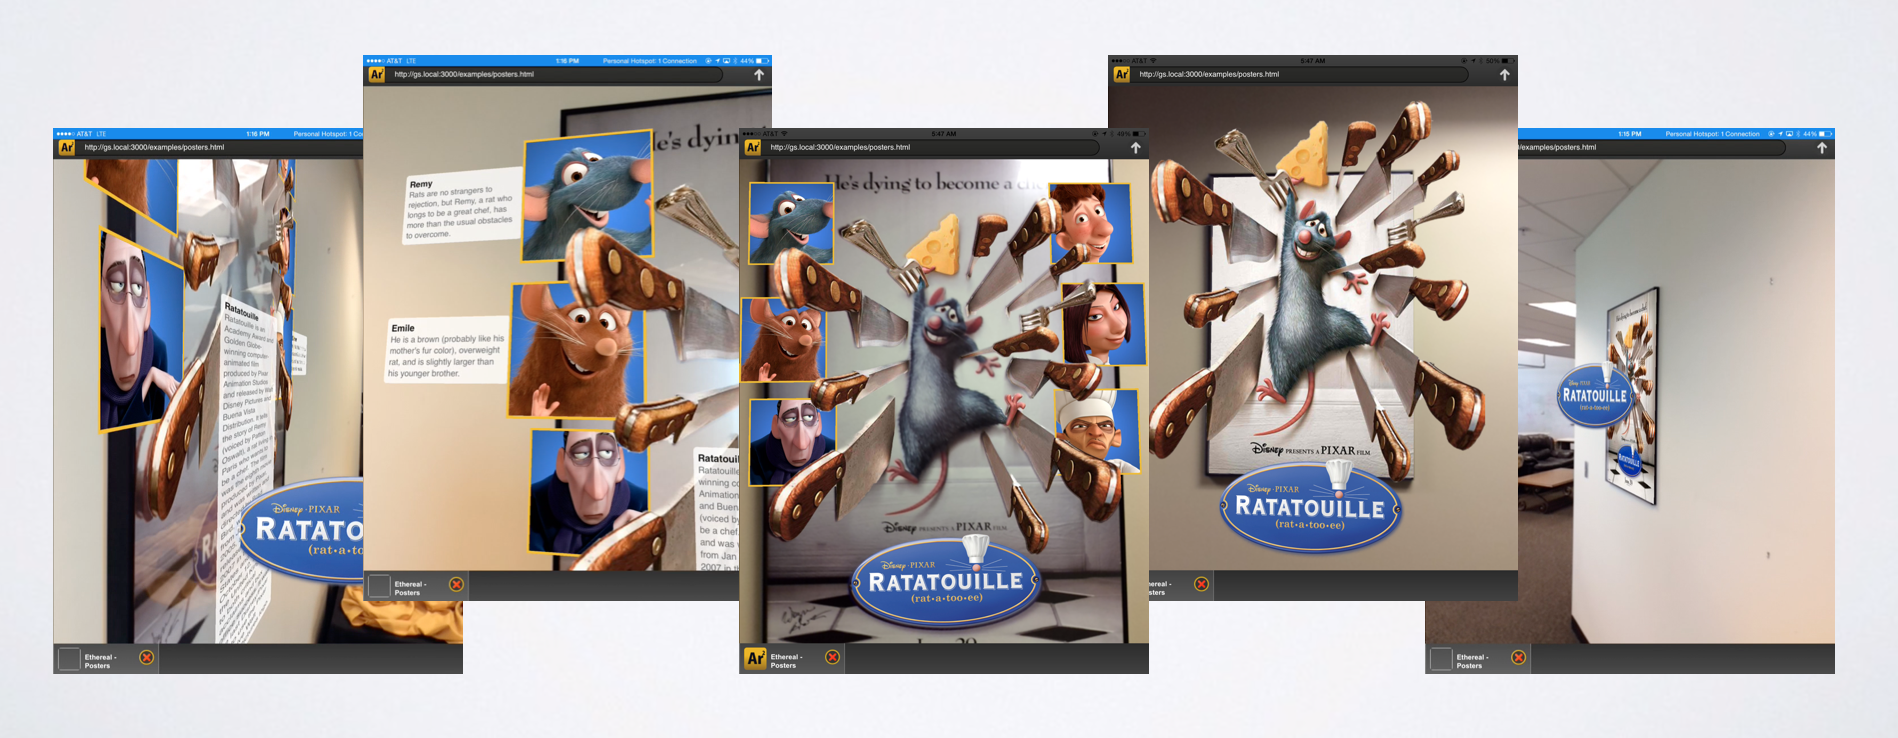
\includegraphics[width=\linewidth]{Ethereal-Demo.png}
  \caption{In this prior work \cite{Speiginer2014Ethereal:Content}, we demonstrated how 2D web content can be used to create interesting, complex, and dynamic 3D UI for augmenting a movie poster (all movie image copyrights belong to Disney). This example relied on CSS 3D Transforms, rather than WebGL (this approach is not feasible for WebXR use-cases, see Section \ref{sec:dom-overlays}).}
  \Description{}
  \label{fig:ethereal}
\end{figure}

This project was created as part of our collaboration with Traclabs\footnote{https://traclabs.com/}, to extend their PRIDE\footnote{https://traclabs.com/projects/pride/} web-based maintenance procedure software to support AR maintenance procedures via WebXR\footnote{The WebXR Device API is the W3C standard for presenting immersive 3D content via web browsers, see https://github.com/immersive-web/webxr} (see Figure \ref{fig:pride}). In this project, we wanted to leverage the layout and styling capabilities of the 2D web for building out various aspects of the user interface, similar to how we have leveraged 2D web technologies for creating 3D UIs in other projects (e.g., see Figure \ref{fig:ethereal}) based on our Argon browser \cite{MacIntyre2011TheEnvironment, Speiginer2015TheApplications}). Argon targeted mobile phones and tablets, and allowed 2D content to be overlaid on a 3D view without rendering the 2D content in 3D, but WebXR requires all content to be presented in 3D via WebGL (to support the full spectrum of immersive displays). Unfortunately, as others have found, there were no adequate solutions for presenting complex interactive 2D web content in a WebGL canvas. This paper is the result of our exploration of various DOM-to-Texture techniques to rasterize bits of web content. We developed  a plugin for three.js (a popular 3D scene-graph library) around an existing DOM-to-Texture library (html2canvas) in order to automate the process of mirroring live DOM elements as interactive layers of rasterized web content within a three.js scene. 

In this section, we review three different kinds of approaches for mixing 2D web content with 3D graphics. 

\subsection{DOM Overlays}
\label{sec:dom-overlays}

A common technique to mix 2D and 3D web content is to overlap a WebGL <canvas> element with other DOM elements. This is the technique we used in Argon, and is a conceptually straightforward method for adding Heads-Up-Display UI to 3D scenes. Using CSS 3D Transforms, it is also possible to visually position DOM elements within the 3D scene.
% (using the same perspective projection as the 3D scene). 
% Some scene-graph libraries (e.g., three.js) even make this kind of technique relatively easy to setup. 
One of the limitations is that multi-viewport rendering (e.g., stereoscopic) requires duplicating DOM elements for each view. Another limitation is that 3D graphics and overlaid 3D Transformed DOM elements are still rendered by entirely different mechanisms, making it difficult to integrate them in complex ways (e.g., applying custom lighting/shadows to DOM elements, handling occlusions between DOM elements and 3D graphics, etc.). The biggest limitation of this approach is that all current Head-Mounted-Displays (HMDs) will only present what is rendered to a WebGL \verb|<canvas>| element, and the underlying system will not easily support overlaying 2D DOM elements.

\subsection{DOM-to-Texture}

The Chrome GPU team\footnote{SIGGRAPH2017 WebGL BOF, www.youtube.com/watch?v=dAtdE4LQCSc\&t=1540} and the Servo Browser team\footnote{Implemented in this PR to Servo https://github.com/servo/servo/pull/18592} have both experimented with implementing APIs for rendering \verb|<iframe>| elements to a WebGL texture and for forwarding input events to the underlying DOM elements from a WebGL canvas. There is no indication, however, that the proposed extension to support such capabilities\footnote{https://www.khronos.org/registry/webgl/extensions/proposals/ WEBGL\_texture\_source\_iframe/} is on a track to ship in any browser, due to security and privacy concerns.  The WebXR community group is also discussing such capabilities\footnote{https://github.com/immersive-web/webxr/issues/400}, but it is unclear if a general, usable solution will be found. 
Until a native DOM-to-Texture solution is available, workarounds have been developed using one of two strategies: placing HTML content within SVG via a \verb|<foreignObject>| element and encoding the resulting markup as a data URI assigned to an Image element (e.g., rasterizeHTML\footnote{https://cburgmer.github.io/rasterizeHTML.js/}); or recreating the rendering logic that the browser uses (e.g., html2canvas\footnote{http://html2canvas.hertzen.com}). 

The advantage of the \verb|<foreignObject>| strategy is that the browser can perform the rasterization (and do it accurately), however the disadvantages are that no external resources are permitted (CSS, JavaScript, and images must all be in-lined and base64 encoded), and browser security restrictions can prevent the resulting image from being readable. The html2canvas library works around these restrictions by performing the rendering itself, however it does not implement all the CSS properties supported by the browser. Various libraries for rendering 2D web content with WebGL (e.g., HTMLGL\footnote{http://htmlgl.com}, html2three\footnote{https://github.com/marciot/html2three}, etc.) have been implemented using these DOM-to-Texture strategies; nevertheless, these were insufficient for our use-case, either supporting a limited scene-graph representation (rasterizing large portions of the DOM, rather than partitioning it into small independently manipulable pieces), or being designed primarily for applying effects to elements on a 2D web page (e.g., HTMLGL).

\subsection{DOM-to-3D}

Marx et al. have experimented with DOM-to-Texture solutions presented above, concluding that existing techniques were not performant enough for the VR use-cases they envisioned \cite{Marx2017DOM2AFRAME:WebVR}. Their solution was to re-create each DOM-element as an individual 3D object in the scene, packaged as a library named DOM2AFRAME.

The approach we present in this paper is at a high-level very similar to DOM2AFRAME, with a shared motivation to support complex 3D UIs built on traditional web technologies; however, our approach reconsiders DOM-to-Texture techniques. Similar to DOM2AFRAME and unlike other DOM-to-Texture solutions (e.g., html2three, HTMLGL, etc.), our approach is designed to support non-trivial arrangement of web content in 3D. While DOM2AFRAME makes it possible to manipulate complex web content in 3D, it accomplishes this by representing every DOM element as a 3D object, making it less scalable than our approach---which offers as much flexibility with less complexity in the 3D scene, easily being capable of presenting complex interactive web content in 3D at maximum frame-rates on modern devices (including mobile). Finally, while DOM2AFRAME attempts to tackle the problem of presenting arbitrary web pages in 3D, we explicitly consider this to be a non-goal. 


\section{WebLayer3D}
As mentioned above, WebLayer3D is designed to expose DOM content as objects within the popular \textif{three.js} graphics library. By encapsulating the framework within a \verb|WebLayer3D| class that extends the core three.js \verb|Object3D| class, web content can be manipulated via three.js's scene-graph representation. Our WebLayer3D library makes it easy to partition a complex DOM tree into multiple layers of individually rasterized web content (with heuristics to determine when any layer needs to be refreshed), allowing web content to be manipulated in 3D in non-trivial ways. Until secure DOM-to-Texture is supported natively, we rely on html2canvas in order to rasterize DOM elements (although, as an optimization, we use only the internal drawing routines, rather than using the library as intended). While html2canvas does not perfectly rasterize the DOM (it does not support many CSS properties), it implements enough to provide a high degree of functionality.

Since a single \textit{web layer} (i.e., a \verb|WebLayer3D| instance) can represent a complex collection of DOM elements, the three.js scene-graph representation can be much simpler than its DOM counterpart. The complexity is entirely dependent on how the designer wishes to arrange the 3D layout of web layers, matching as much or as little of the structure of the respective DOM tree.  A key benefit of this layered approach is that rasterization can be performed on each layer independently, avoiding the potential performance bottleneck from rasterizing the entire DOM tree every time a sublayer needs to be refreshed. By maintaining a live connection to the DOM, we are able to keep each web layer refreshed whenever the DOM changes, while also supporting interaction with the underlying DOM elements via the 3D scene. For example, our approach supports interaction with form <input> elements (e.g., text input, checkboxes, etc.), no matter where their respective layers are positioned in the 3D scene. 


\begin{listing}[H]
\caption{Basic Setup}
\label{listing:basic-setup}
\begin{minted}[mathescape,
               linenos,
               numbersep=5pt,
               frame=lines,
               framesep=2mm]{javascript}
// create the WebLayer3D instance
const rootLayer = new WebLayer3D(domElement, {
    // the following parameters are optional
    pixelRatio: window.devicePixelRatio,
    layerSeparation: 0.001,
    onLayerCreate: (layer) => {
        // do something every time a layer is created
        // e.g., attach a cursor mesh
        const sphere = new THREE.Sphere(0.01)
        layer.cursor.add(new THREE.Mesh(sphere))
    }
}) 
// add to three.js scene
scene.add(rootLayer)
// setup interaction rays for hover state 
rootLayer.interactionRays = [mouseRay]
renderer.domElement
        .addEventListener('mousemove', (e) => {
    updateMouseRay(e)
})
// setup hit testing
renderer.domElement
        .addEventListener('click', (e) => {
    updateMouseRay(e)
    const hit = rootLayer.hitTest(mouseRay)
    if (hit) {
        const newEvent = new e.constructor(e.type, e)
        hit.target.dispatchEvent(newEvent)
    }
}
// update in animation loop
function animate() {
    // ...
    // update pose, visibility, and textures 
    // on each layer
    rootLayer.update()
}
\end{minted}
\end{listing}

\subsection{Basic Setup}

After setting up the three.js scene, a developer simply creates a new \verb|WebLayer3D| instance, passes in the desired DOM element, and associates interaction rays with the root layer. During initialization, the \verb|WebLayer3D| instance will traverse the DOM tree, and any child elements that possesses a \verb|data-layer| attribute will be added as a child \verb|WebLayer3D| instance. Each time through the animation loop, \verb|update()| should be called on the root WebLayer3D object, which will update the layout of the entire layer hierarchy, automatically adapting to changes in the DOM (including addition or removal of DOM elements), and updating textures as needed. This basic setup is summarized in the code sample in Listing~\ref{listing:basic-setup}. (In this setup, the \verb|mouseRay| and hit testing are based on a mouse or touch display; an immersive display would use 3D input to update one or more interaction rays and to perform hit testing [see Section \ref{sec:rays}.]) 



\subsection{Annotating and Styling Web Content}
\label{sec:annotating}

The DOM can be annotated with special data attributes to specify how the DOM tree should be partitioned and rasterized. These attributes can be included directly in the HTML (see Listing~\ref{listing:annotations-HTML}), or can be dynamically set via standard DOM APIs (see Listing \ref{listing:annotations-JS}).

\begin{listing}[H]
\caption{Annotating the DOM via HTML}
\label{listing:annotations-HTML}
\begin{minted}[mathescape,
               linenos,
               numbersep=5pt,
               frame=lines,
               framesep=2mm]{html}
<ul data-layer data-layer-pixel-ratio="0.5">
<li><div data-layer><image src="..."/>Item</div></li>
<li><div data-layer><image src="..."/>Item</div></li>
<li><div data-layer><image src="..."/>Item</div></li>
</ul>
\end{minted}
\end{listing}

\vspace{-12px}

\begin{listing}[H]
\caption{Annotating the DOM via JavaScript}
\label{listing:annotations-JS}
\begin{minted}[mathescape,
               linenos,
               numbersep=5pt,
               frame=lines,
               framesep=2mm]{javascript}
const list = document.querySelector('ul')
list.dataset.layer = ''
list.dataset.layerPixelRatio = '0.5'
const innerDivs = list.querySelectorAll('li div')
for (div of innerDivs) div.dataset.layer = ''
\end{minted}
\end{listing}

The following are the full set of attributes we support: 

\subsubsection{data-layer}
The \verb|data-layer| attribute is implied for the root element. When WebLayer3D encounters this attribute in a child element, it prevents that element from being rasterized within the current layer (hiding that element and its descendants), and rasterizes it within a new WebLayer3D instance that is added as a child of the current layer. After a WebLayer3D instance is created, this attribute is set to a number that corresponds with the \verb|id| of the layer (inherited from the three.js \verb|Object3D| class). 

\subsubsection{data-layer-pixel-ratio}
This attribute allows the author to scale the pixel ratio of a layer independently from other layers (the default pixel ratio is the device's native pixel ratio, and can be overridden for all layers in the options dictionary passed to the \verb|WebLayer3D| constructor). Some elements, particularly container elements that provide only a background for other content, may receive very little benefit from a large pixel ratio, so scaling it down can save texture memory without impacting the resulting visual fidelity or readability of content (e.g., text) in child layers. 

\subsubsection{data-layer-hover-depth}
While \textit{hover states} are natively supported in browsers (via the \verb|:hover| pseudo-class), the DOM supports no mechanism for manipulating or observing the hover state of DOM elements. To support hover states for 3D, we require authors to specify how many hover states are required for a given layer (by setting an integer value on the \verb|data-layer-hover-depth| attribute, which defaults to 0). The reason multiple hover states may be needed is because it is common for hovers on parent elements to affect the style of child elements differently than a direct hover on that child element. Styling hover states for 3D is relatively straightforward, and only requires modifying CSS to use a \verb|hover| class rather than the typical \verb|:hover| pseudo-class. 

Listings \ref{listing:annotations-hover} and \ref{listing:styles-hover} are part of our TodoMVC case study, where we used the \verb|data-layer-hover-depth| attribute to pre-render styles for no hovering, direct hovering, and parent hovering. Note that while our implementation requires developers to use a \verb|hover| class instead of the standard \verb|:hover| pseudo-class, these can be used together in order to support hover states in both the 2D DOM and the 3D scene.

\begin{listing}[H]
\caption{Configuring hover depth}
\label{listing:annotations-hover}
\begin{minted}[mathescape,
               linenos,
               numbersep=5pt,
               frame=lines,
               framesep=2mm]{HTML}
<button class="destroy" data-layer 
        data-layer-hover-depth="2">x</button>
\end{minted}
\end{listing}

\begin{listing}[H]
\caption{Styling hover state}
\label{listing:styles-hover}
\begin{minted}[mathescape,
               linenos,
               numbersep=5pt,
               frame=lines,
               framesep=2mm]{CSS}
/* style for hover state of 0 (no hover) */               
.todo-list .destroy {
	display: none;
	color: #cc9a9a;
}
/* style for hover state of 1 (direct hover) */
.todo-list .destroy:hover, 
.todo-list .destroy.hover {
	color: #af5b5e;
}
/* style for hover state of 2 (parent hover) */
.todo-list li:hover .destroy, 
.todo-list li.hover .destroy {
	display: block;
}
\end{minted}
\end{listing}

\begin{figure}[H]
  \centering
    \begin{subfigure}{0.48\linewidth}
    \centering
    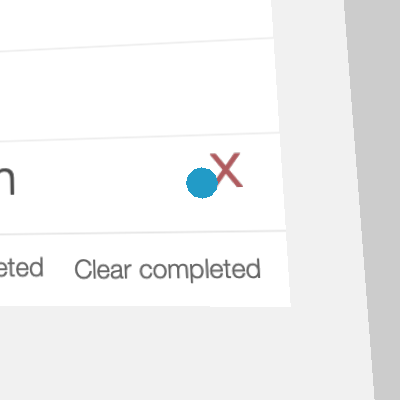
\includegraphics[trim={16px 30px 0 30px},clip, width=\linewidth]{TodoMVC-Hover-1.png}
    \end{subfigure}
    \begin{subfigure}{0.48\linewidth}
    \centering
    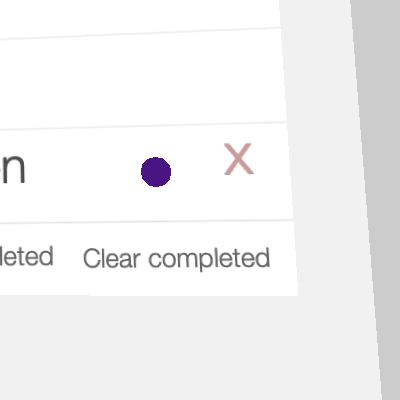
\includegraphics[trim={16px 30px 0 30px},clip, width=\linewidth]{TodoMVC-Hover-2.png}
    \end{subfigure}
  \caption{ The results of the annotation and styling in Listings \ref{listing:annotations-hover} and \ref{listing:styles-hover} . Direct hover shows a bright red X (left) and parent hover shows a light red X (right), changing automatically as interaction rays intersect with layers. The button disappears when there is no hover. Each layer is assigned a different cursor for demonstration purposes (here, the cursor color is blue when directly over the button layer, and changes to purple when over the parent layer).}
  \Description{}
  \label{fig:hover}
\end{figure}


\subsubsection{data-layer-states}
\label{sec:states}
By default, a \verb|WebLayer3D| object manages a single texture, refreshing it dynamically as the DOM tree is modified (see refresh heuristics in Section \ref{sec:refresh} for details). It is quite common, however, for web content to alternate between fixed visual styles based on the dynamic addition and removal of CSS classes (or pseudo-classes, such as \verb|:hover|). The \verb|data-layer-states| attribute, which expects a whitespace-delimited list (e.g., \verb|"near far"|), is designed to facilitate this adaptive usage of CSS classes (beyond hover states). When these \textit{class states} are specified, they are combined with each hover state, rasterized, and cached as individual textures---eliminating the need to perform rasterization when alternating between these classes. Unlike hover states, which are managed implicitly (via interaction rays, see Section \ref{sec:rays}), class states are managed explicitly by setting or removing classes on the underlying DOM element. Like hover states, each class state can be styled with standard CSS.


\begin{figure}[t]
  \centering
    \begin{subfigure}{0.48\linewidth}
    \centering
    
\includegraphics[trim={16px 30px 0 30px},clip, width=\linewidth]{todo-unchecked.jpg}
    \end{subfigure}
    \begin{subfigure}{0.48\linewidth}
    \centering
    
\includegraphics[trim={16px 30px 0 30px},clip, width=\linewidth]{todo-checked.jpg}
    \end{subfigure}
  \caption{These checkboxes and textboxes in the TodoMVC case study are implemented using the \textit{class states} described in Section \ref{sec:states}, allowing the application to toggle their ``completed'' state on or off without re-rasterizing them.}
  \Description{}
  \label{fig:hover}
\end{figure}

\subsection{Interacting with Web Content}
We support two basic mechanisms for interaction with web content in 3D: deep hit testing and interaction rays. 

\subsubsection{Deep Hit Testing} 
With hit testing, authors can develop interactions based on pointing at web layers. In order to make interacting with the underlying DOM easier, we provide a utility hit testing function that performs hit testing not only on the 3D layers, but also on their underlying DOM elements (in order to retrieve the exact DOM element that was hit). Authors are free to react to a hit test in any number of ways: simulating 3D physics forces on the hit layer, applying or removing CSS classes on the underlying DOM element, or simply forwarding an event to the underlying DOM element (such an event forwarding strategy is depicted in Listing \ref{listing:basic-setup}, lines 27-28).
\subsubsection{Interaction Rays}
\label{sec:rays}
Interaction rays are the mechanism by which we support the 3D hover state. When authors assign one or more interaction rays to the root layer (and keep them updated each frame), we automatically switch between hover and non-hover textures for all layers in the hierarchy (this mechanism supports interaction with multiple 3D pointers/controllers, as demonstrated in Figure \ref{fig:dualInput}). Hover states are updated (based on the current interaction rays) every time the \verb|update()| function is called on a root layer. While this interaction mechanism relies on hit testing, it does not touch the DOM or require re-rasterizing any layers.

\begin{figure}[h]
  \centering
  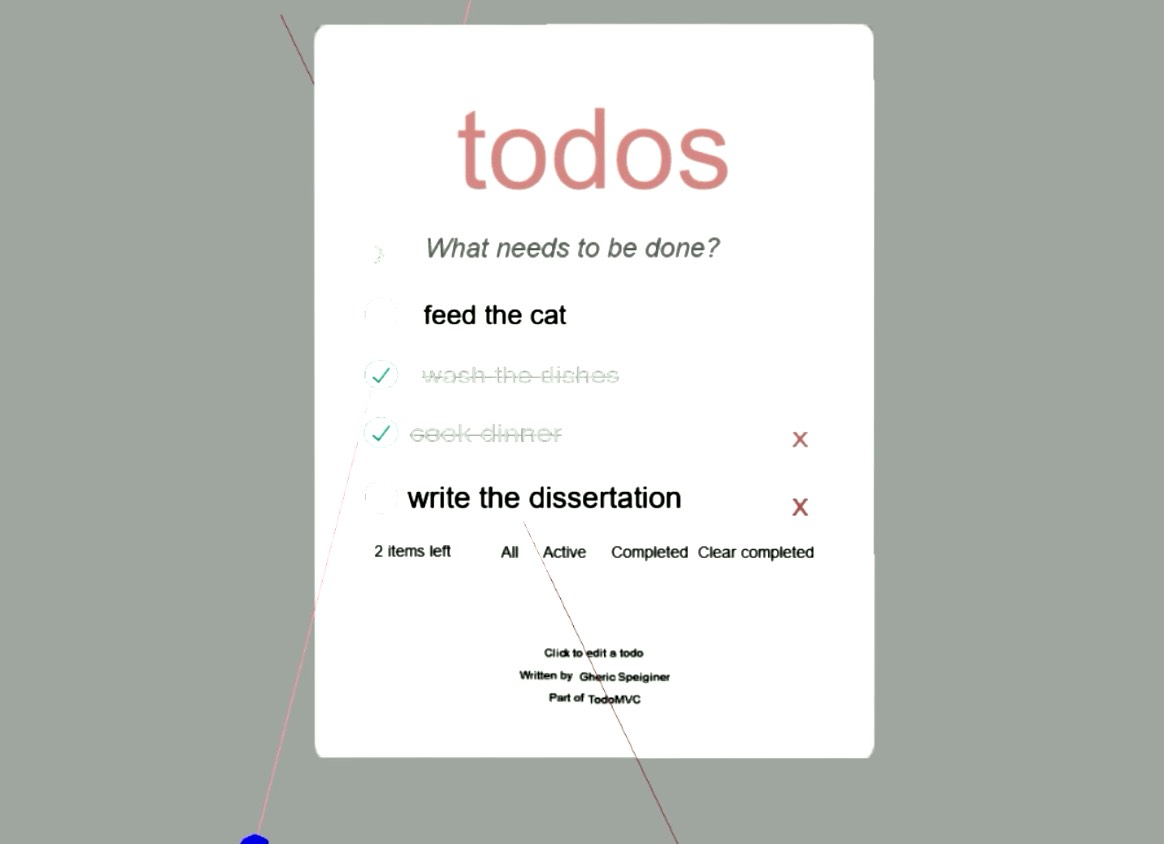
\includegraphics[width=\linewidth]{TodoMVC-dualInput.jpg}
  \caption{TodoMVC in WebVR on a Windows Mixed Reality HMD. Both controllers control separate interaction rays, causing the last two items to show their hover state (the red X on the right end of the line.) }
  \Description{}
  \label{fig:dualInput}
\end{figure}

\subsection{Updating and Rasterizing Web Content}

Our library expects users to call an \verb|update| method, each frame, to keep web layers in sync with the underlying DOM and to maintain various properties in their correct state (i.e., interaction ray hits, hover states, textures, etc.). This \textit{update} routine traverses the underlying DOM tree in order to maintain a representation of the current DOM layout. Since there is currently no straightforward way to know when DOM layout (or styles) have changed, we take a safe approach and capture the computed layout each frame---unfortunately, while capturing layout calculations is feasible, capturing and parsing the multitude of computed styles available in modern browsers is the primary bottleneck for libraries like html2canvas, and is not practical to perform continually for each layer. Nevertheless, by using several heuristics to signal that styles (may) have changed, splitting rasterization work across layers, and scheduling that work between frames, our \textit{update} and \textit{rasterize} routines are carefully optimized for complex interactive UIs. 

%  When rasterizing a layer element with html2canvas, we (temporarily) set the \verb|opacity| to 0 on child layer elements to exclude their content from the resulting texture. 

\subsubsection{Refresh Heuristics} 
\label{sec:refresh} In order to determine when a layer needs to be refreshed, we rely on a set of heuristics based on observing changes to the DOM. This includes watching for text and attribute changes within DOM elements (via \verb|MutationObserver|), watching for elements that are resized (via \verb|ResizeObserver|), and watching for DOM events that signal user input (such as \verb|input| and \verb|change| events). Based on these heuristics, we schedule a layer for asynchronous rasterization by adding it to a queue to be processed at an appropriate time. Normally, modifying any DOM attribute would cause our heuristics to trigger a refresh on the containing layer; however, when the added/removed CSS class is a known layer state (see Section \ref{sec:states}), we skip the rasterization process and simply switch to the appropriate cached texture.

\subsubsection{Scheduling Rasterization}
Since our approach is tied to the DOM, all rasterization work is performed on the main thread; therefore, we are careful to schedule this work such that any impact on the framerate is minimized. For example, any pending work is split into smaller tasks (one task per layer), which are scheduled to be processed asynchronously, between frames. This processing continues until there are no more tasks, or until a certain amount of time has passed (rasterization tasks can be processed across multiple frames, if necessary). When available, we rely on the \verb|requestIdleCallback| API in order to flexibly schedule these tasks during idle CPU times (taking into account a browser-provided idle deadline); otherwise, as a fallback, we schedule these tasks to run immediately after the current frame has rendered, allocating a maximum of 5 milliseconds per frame (based on a target frame rate of 60 FPS, or a maximum budget of 16 milliseconds per frame).


\subsection{Manipulating Web Content in 3D}
Our WebLayer3D library includes support for transitioning the layout and visibility of web content (e.g., linearly interpolating the position, size, and opacity of layer objects as the underlying DOM structure changes), and enables authors to modify how layers are transitioned from layout to layout. We provide default transition functions which can be overridden at varying levels of abstraction, or completely replaced with custom layout logic. Furthermore, authors can easily combine the use of traditional web capabilities with application-specific 3D spatial reasoning (e.g., mixing together 2D and 3D layout algorithms, using semantic DOM queries in combination with 3D proxemics, etc.). For example, in the TracLabs case study, we mix 3D force-directed layout with standard 2D web layout (see Figure \ref{fig:pride}, right). The code sample in Listing \ref{listing:modifylayout}, taken from our TodoMVC case study, shows how we combine the use of CSS selectors and hover states derived from 3D interaction rays in order to apply a hover effect to individual layers in the 3D scene.


\begin{listing}[H]
\caption{Customized Layer Updates}
\label{listing:modifylayout}
\begin{minted}[mathescape,
               linenos,
               numbersep=5pt,
               frame=lines,
               framesep=2mm]{javascript}
todoLayer.update(lerpValue, (layer, alpha) => {
    // modify the z distance between layers
    layer.contentTarget.position.z  = 
      Controls.layerSeparation * layer.level
    // apply a hover effect (move forward and grow)
    // to certain layers
    if (Controls.hoverEffect) {
      if (
        layer.hover === 1 &&
        layer.level > 1 &&
        !layer.element.matches('h1') &&
        !layer.element.matches('.todo-count')
      ) {
        layer.contentTarget.position.z += 
          Controls.layerSeparation * 0.3
        layer.contentTarget.scale.multiplyScalar(1.1)
      }
    }
    // transition layout & visibility to target values
    WebLayer3D.TRANSITION_DEFAULT(layer, alpha)
  })
\end{minted}
\end{listing}

% We achieve this flexibility by (1) decoupling the \textit{actual} layout from a \textit{target} layout (modelled on the current DOM layout), (2) providing a sensible default behavior for transitioning the current layout to a target layout, and (3) allowing this default behavior to be customized or overridden at multiple levels of abstraction.

% For instance, all WebLayer3D instances have a \verb|targetContentPosition| and a \verb|targetContentScale| that is set to match the DOM's layout calculations each time the \verb|update()| function is called on a root web layer.

% TODO: ADD MORE DETAILS, CODE, AND SHOW SOME CUSTOM SPATIAL LAYOUTS

\subsection{Evaluating Performance}
To evaluate the performance of our approach, we profiled our \textit{update} and \textit{rasterize} routines in our WebLayer3D library (while running the TodoMVC case study with 50+ \verb|WebLayer3D| instances), on a base-model 2018 MacBook Air (8 GB RAM, 1.6 GHz Intel Core i5, Intel UHD Graphics), a high-performance VR-capable PC (32 GB RAM, 3.6 GHz AMD Ryzen 7 1800X, NVIDIA GeForce GTX 1080), and an iPhone XS. In all of our test cases, we achieved a steady 60 or 90 frames per second (FPS), with plenty of spare milliseconds for other application logic. 

On the MacbookAir, we ran the TodoMVC example in Safari 12.1, Chrome 73, and Firefox 66 (all running at 60 FPS). The \textit{update} routine averaged 2.7 to 3.3 ms per frame (for 50+ layers), and the \textit{rasterize} routine (which only runs when rasterizations are queued) averaged 3.8 ms per layer on Safari (averaging 1.8 layers per post-render allocation period of 5ms), 5.8 ms per layer on Chrome (averaging 1.4 layers per idle callback), and, 3.7 ms per layer on Firefox (averaging 2.2 layers per idle callback). Notably, the amount of time that html2canvas spends actually drawing to a canvas is virtually negligible; the bulk of this "rasterization" time is spent traversing the DOM to retrieve and parse the current computed style/layout values.
On the PC, we ran the TodoMVC demo in Firefox 66 while presenting to a Windows Mixed Reality head-worn display (DELL Visor VR118) and interacting with two 6DOF controllers, at a steady 90 frames per second. On this system, the \textit{update} routine averaged 1.6 ms, and the \textit{rasterize} routine averaged 2.2 ms per layer (averaging 6 layers per idle callback). Finally, running at 60 FPS on the iPhone XS, the \textit{update} routine took an average of 1.2 ms per frame, and the \textit{rasterize} routine took an average of 2.6 ms per layer (averaging 2 layers per post-render allocation period of 5ms). 

\subsection{Limitations}
Some limitations are inherent to our use of html2canvas, which has limited (though generally sufficient) CSS styling support, and can be slow when rasterizing many layers at once (hence our efforts to make sure rasterization is only performed when necessary). Since html2canvas is designed for taking screenshots, the library is not optimized for real-time use---by default, html2canvas clones the entire DOM tree each time it is called. For our use case, we found that cloning the DOM tree is unnecessary, and are thus only relying on the library's internal rendering routines. We also encountered issues with rasterizing content styled with pseudo-elements or CSS Transforms---although these specific issues were likely related to our avoidance of the public html2canvas API. These particular limitations with html2canvas would become irrelevant if browsers provided secure native DOM rasterization. 

Other limitations are inherent to our overall approach: the built-in scrolling/overflow mechanism in the DOM would not be trivial to implement in 3D (the authors of DOM2AFRAME have documented the difficultly of doing so), and our approach is generally not intended to support interaction with arbitrary 2D web content. Due to limitations inherent in both html2canvas and in our approach, content outside of the border-box\footnote{The border-box includes the content, padding, and border of a DOM element} of a layer's DOM element is not rasterized at all (note that Figure \ref{fig:teaser} (b) does not display the box-shadow styles from Figure \ref{fig:teaser} (a)). Finally, because current browser API's do not provide a reliable mechanism for detecting when styles have changed on an arbitrary element, there are many cases where our heuristics will not trigger a refresh even though the DOM presentation may have changed (e.g., cascading styles that affect presentation of content in adjacent layers without affecting their layout), or where a refresh may be triggered when it wasn't necessary (e.g. a CSS class applied on parent element that only affects elements in child layers). In general, working around these refresh issues is relatively straightforward, either by tweaking CSS rules, changing how the DOM is partitioned into 3D layers, or manually triggering refreshes in cases where the heuristics fail. Furthermore, future Web APIs\footnote{https://developers.google.com/web/updates/2016/05/houdini} should enable more robust and performant detection of changes in both layout and presentation of DOM elements. 

\begin{figure}[h]
  \centering
  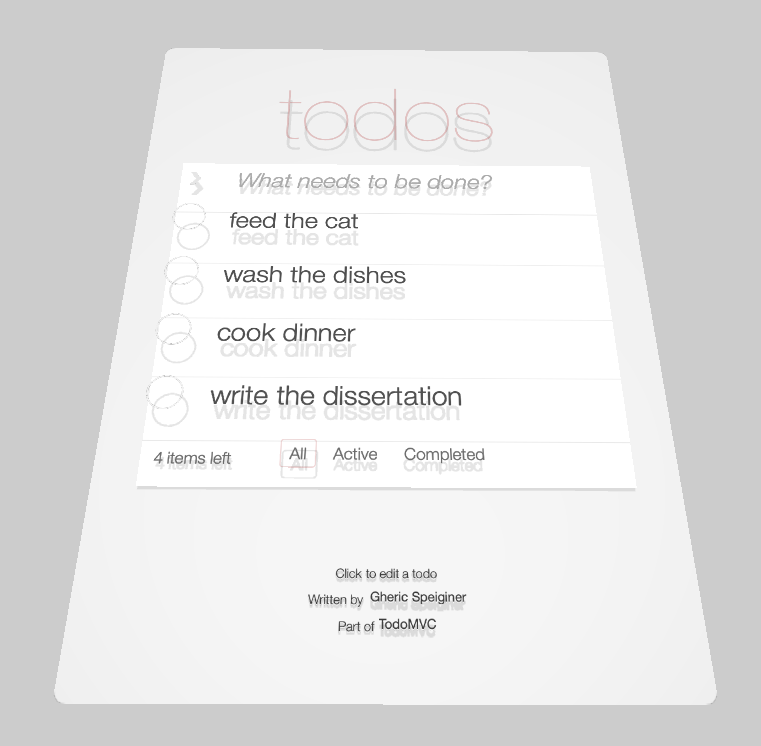
\includegraphics[width=\linewidth]{TodoMVC-Shadows-2.png}
  \caption{TodoMVC with 3D lighting and shadows}
  \Description{}
  \label{fig:todo-shadows}
\end{figure}

\section{Case Studies}

We have implemented two different case studies using our WebLayer3D library, both of which rely on Vue.js for reactive data-binding and for managing updates to the DOM (via a virtual DOM), and three.js for rendering the 3D scene (via WebGL). 

\subsection{TodoMVC in 3D}
This case study implements the canonical TodoMVC example\footnote{http://todomvc.com/}, an example web-app specification expressly designed to demonstrate the pros and cons of particular web frameworks.  TodoMVC has been implemented hundreds of times using a wide variety of popular web frameworks. What sets our implementation apart from other implementations (to the best of our knowledge) is that our version runs in WebGL, using the approach we have presented in this paper. In order to create a version of TodoMVC that leveraged our library, we started with a typical TodoMVC implementation (written using the Vue.js framework), and modified it in the following ways:
\begin{itemize}
\item Added three.js scene and render loop for rendering to WebGL and leveraging WebVR/WebXR tracking capabilties. 
\item Annotated DOM elements with special attributes (as described in Section \ref{sec:annotating}), while adjusting the structure of the DOM slightly to segment content within certain layers for demonstration purposes. 
\item Modified styles on the \verb|h1| header element to ensure all of the text was contained within the border-box (otherwise, the text would have been clipped). 
\item Changed checkbox SVG images encoded in data urls (embedded in CSS) to SVG images embedded in HTML (due to security errors in Safari when rasterizing data uri images with html2canvas).
\item Added \verb|hover| class selectors to CSS (where there were previously only \verb|:hover| psuedo-class selectors).
\item Removed psuedo-element rules from CSS (for rendering check box images), replaced with actual DOM elements (because we use html2canvas in a non-standard way, pseudo-elements failed to rasterize properly).
\item Adjusted CSS rules and data-binding logic to isolate the use of cascading styles within invidual layers (in order to support pre-rendered class states, as described in Section \ref{sec:states}).
\item Added dynamic layout for 3D interaction (e.g., hover effects).
\item Added experimental lighting and shadows (see Figure \ref{fig:todo-shadows}).
\end{itemize}



\subsection{PRIDE System AR Interface}
\label{section:pride}
The PRIDE system AR interface is a realistic example work-in-progress that extends an existing maintenance procedure system for AR use-cases while exploring what it means to build complex 3D UIs that can effectively adapt to a range of hardware configurations and environment conditions. Like the TodoMVC case study, we are using Vue.js for data-binding and managing the DOM state.


\section{Future Work}
The library supports the core features required to add 2D DOM content into 3D WebGL and WebXR UIs, but there are various opportunities to increase performance and add more capabilities.  For example, the library automatically supports video playback by recognizing \verb|<video>| tags and using three.js to render the video element directly to a texture (using support already in three.js). Other opportunities for more tightly integrating 2D elements in 3D likely exist.

Recall that our approach is motivated by a desire to support the design of 3D UI for various XR devices and use-cases. While we are using the library in our work on the PRIDE system (see Section \ref{section:pride}), we have not yet used it in other examples, or created more than the simple TodoMVC example on an immersive HMD.  We are particularly interested in integrating this library with more elaborate 3D widget libraries for three.js, and with exposing these capabilities into libraries built on top of three.js, such as AFrame\footnote{https://aframe.io}. We plan on exploring the potential for this approach by replacing some of the dat.gui-based\footnote{https://github.com/dataarts/dat.gui} UIs in various three.js demos with richer 2D UIs that also work in WebXR. 

\section{Conclusion}
In this paper, we have demonstrated that existing DOM-to-Texture techniques (when used thoughtfully) can enable a performant, simple, and powerful approach for leveraging traditional web capabilities to build complex interactive 3D UI on the immersive web. A native DOM-to-Texture capability in browsers would improve the fidelity and performance of this approach---nevertheless, by leveraging libraries such as html2canvas, the approach we have described is viable today. 



%
% The acknowledgments section is defined using the "acks" environment (and NOT an unnumbered section). This ensures
% the proper identification of the section in the article metadata, and the consistent spelling of the heading.
% \begin{acks}
% To Robert, for the bagels and explaining CMYK and color spaces.
% \end{acks}


\begin{acks}
  The authors would like to thank 
%   AT\&T, Alcatel-Lucent, Qualcomm, Mozilla, 
  TracLabs and NASA for their support of this project.  The authors are supported by a NASA SBIR with TracLabs.
%   in addition to Taeheon Kim and all the students, researchers and sponsors who used (and supported those using) the Argon platform. 
We have benefited from ongoing support from the GVU Center at Georgia Tech, and from the support of the NSF Graduate Research Fellowship and the GEM fellowship for the first author.
\end{acks}

%
% The next two lines define the bibliography style to be used, and the bibliography file.
\bibliographystyle{ACM-Reference-Format}
\bibliography{mendelay}

% 
% If your work has an appendix, this is the place to put it.
% \appendix

% \section{Research Methods}

% \subsection{Part One}

% Lorem ipsum dolor sit amet, consectetur adipiscing elit. Morbi malesuada, quam in pulvinar varius, metus nunc fermentum urna, id sollicitudin purus odio sit amet enim. Aliquam ullamcorper eu ipsum vel mollis. Curabitur quis dictum nisl. Phasellus vel semper risus, et lacinia dolor. Integer ultricies commodo sem nec semper. 

% \subsection{Part Two}

% Etiam commodo feugiat nisl pulvinar pellentesque. Etiam auctor sodales ligula, non varius nibh pulvinar semper. Suspendisse nec lectus non ipsum convallis congue hendrerit vitae sapien. Donec at laoreet eros. Vivamus non purus placerat, scelerisque diam eu, cursus ante. Etiam aliquam tortor auctor efficitur mattis. 

% \section{Online Resources}

% Nam id fermentum dui. Suspendisse sagittis tortor a nulla mollis, in pulvinar ex pretium. Sed interdum orci quis metus euismod, et sagittis enim maximus. Vestibulum gravida massa ut felis suscipit congue. Quisque mattis elit a risus ultrices commodo venenatis eget dui. Etiam sagittis eleifend elementum. 

% Nam interdum magna at lectus dignissim, ac dignissim lorem rhoncus. Maecenas eu arcu ac neque placerat aliquam. Nunc pulvinar massa et mattis lacinia.

\end{document}
